\documentclass[superscriptaddress,unsortedaddress,amsmath,amssymb,aps]{revtex4-2}

\usepackage{graphicx}
\usepackage{dcolumn}
\usepackage{bm}
\usepackage{physics}
\usepackage{lipsum}
\usepackage{adjustbox}

%\usepackage{subfig}
\usepackage{braket}
%\usepackage{subcaption}

\usepackage{booktabs}
\usepackage{bm}

\usepackage[utf8]{inputenc}
\usepackage[caption=false,font=small]{subfig} % REVTeX-safe
\newlength{\figgutter}
\setlength{\figgutter}{0.3em}
% Width of each panel (slightly under 1/3 to avoid rounding/spacing issues)
% Width for a 2-column subfloat grid inside figure*
% 2-column grid panels: control HEIGHT so the 4x2 figure fits on the page
% Width for 2x2 grids inside a two-column figure*
\newcommand{\twogridw}{0.49\textwidth}
\newcommand{\densimgtwo}[1]{%
  \includegraphics[width=\twogridw, trim=10mm 8mm 10mm 8mm, clip]{#1}%
}


\newcommand{\threecolw}{0.327\textwidth}
\usepackage{makecell}

\usepackage[flushleft]{threeparttable}  % provides the threeparttable and tablenotes environments

% Crop helper (trim = left bottom right top). Tweak numbers if needed.
\newcommand{\densimg}[1]{%
  \includegraphics[width=\threecolw, trim=10mm 8mm 10mm 8mm, clip]{#1}%
}




\begin{document}

\title{Physics-informed Neural Networks and properties of Quantum Dots Systems}



\author{Morten Hjorth-Jensen}
\affiliation{Department of Physics and Center for Computing in Science Education, University of Oslo, N-0316 Oslo, Norway}



\date{\today}


\maketitle

\section{Introduction}

%{\bf references will be added and more rewrites will come.}\newline

Semiconductor quantum dot systems constitute one of the most versatile
and controllable platforms for studying quantum mechanical many-body
phenomena. Often referred to as artificial atoms, quantum dots allow
for precise tuning of particle number, confinement geometry,
interaction strength, and coupling to external fields through
electrostatic gates and heterostructure design. This high degree of
experimental control has positioned quantum dots at the intersection
of condensed matter physics, quantum information science, and
nanotechnology, enabling systematic investigations of correlation
effects, coherence, and nonequilibrium dynamics at the nanoscale.

From a theoretical perspective, quantum dots provide a clean
realization of interacting fermionic systems in reduced dimensions,
where Coulomb interactions, exchange effects, and quantum confinement
all play essential roles. Even for a small number of particles, the
interplay between single-particle shell structure and many-body
correlations leads to rich physical behavior, including Wigner
molecule formation, spin ordering, and nontrivial excitation
spectra. As the system size increases, the Hilbert space grows
combinatorially, rendering exact solutions intractable and placing
quantum dot systems squarely within the broader challenge of quantum
many-body physics.

Traditional theoretical approaches such as exact diagonalization,
configuration interaction, quantum Monte Carlo, density functional
theory, and mean-field or perturbative methods, have each achieved
notable success in specific regimes. However, these methods face
intrinsic limitations. Exact diagonalization is restricted to very
small particle numbers, Monte Carlo methods may suffer from the
fermion sign problem, and approximate schemes often rely on
uncontrolled assumptions that limit their predictive power in strongly
correlated or nonequilibrium regimes. These challenges are exacerbated
when one seeks to explore high-dimensional parameter spaces, optimize
device geometries, or model realistic experimental conditions.

In recent years, machine learning and neural-network–based approaches
have emerged as powerful complementary tools for tackling complex
problems in quantum many-body physics. Neural networks offer flexible,
high-dimensional function representations that can efficiently capture
nontrivial correlations and emergent structures. Notable examples
include neural-network quantum states, autoregressive wave-function
models, and hybrid schemes combining variational principles with deep
learning. These methods have demonstrated remarkable expressivity,
often achieving accuracies comparable to or exceeding traditional
variational ansätze.

Within this broader context, physics-informed neural networks (PINNs)
provide a particularly promising framework for quantum dot
studies. Unlike purely data-driven models, PINNs embed physical laws,
symmetries, and constraints directly into the learning process,
typically by incorporating differential equations, boundary
conditions, conservation laws, and known operator structures into the
loss function. For quantum systems, this allows the Schrödinger
equation, many-body Hamiltonians, and symmetry requirements, such as
antisymmetry under particle exchange, to guide the optimization of
neural representations.

Applied to quantum dot systems, PINNs offer several compelling
advantages. First, they enable the direct solution of many-body
Schrödinger equations in continuous space without reliance on
predefined basis sets, mitigating basis truncation errors. Second,
they naturally accommodate complex geometries and external potentials,
making them well suited for realistic device modeling. Third, by
employing physical constraints, PINNs often require significantly
less training data than conventional neural networks, improving
interpretability and robustness. Finally, PINNs provide a unified
framework capable of interpolating between few-body and many-body
regimes, as well as between equilibrium and time-dependent dynamics.

The integration of physics-informed machine learning with quantum dot
many-body theory thus represents a promising pathway toward overcoming
longstanding computational barriers. Beyond providing efficient
numerical solvers, these approaches open new avenues for discovering
emergent structure, identifying effective degrees of freedom, and
accelerating design and control of quantum devices. As quantum dot
platforms continue to mature experimentally, the development of
scalable, physically grounded theoretical methods will be essential
for fully exploiting their potential in quantum simulation, quantum
computation, and nanoscale electronics.


{\bf to be rewritten, old text pasted in here}\newline
by minimizing the expectation value of the Hamiltonian using Monte
Carlo sampling. Prominent examples include restricted Boltzmann
machines, feed-forward networks, and more recently deep convolutional
or transformer-based architectures. VMC methods are firmly rooted in
the variational principle and are particularly effective for
ground-state problems. However, they rely on stochastic sampling in
configuration space, which can become computationally expensive in
high dimensions or for fermionic systems with complex nodal
structures. Moreover, the quality of the results depends sensitively
on the chosen sampling strategy and the expressivity of the neural
ansatz, and extensions to excited states or real-time dynamics remain
challenging.

Autoregressive neural states (ANS) address some of these limitations
by representing the wave function as a product of conditional
probability amplitudes, enabling exact and unbiased sampling without
Markov chains. This eliminates autocorrelation issues and
significantly improves training stability. Autoregressive models have
demonstrated impressive performance for lattice systems and discrete
degrees of freedom, and they are particularly well suited for
large-scale variational calculations. However, their application to
continuous-space systems, such as quantum dots with realistic
confinement potentials, is less straightforward and often requires
nontrivial discretization or coordinate transformations. In addition,
like VMC, autoregressive approaches remain fundamentally variational
and typically focus on stationary states.

In contrast, physics-informed neural networks (PINNs) take a
conceptually different approach. Rather than optimizing a variational
energy functional via stochastic sampling, PINNs incorporate the
governing physical equations directly into the loss function,
enforcing the many-body Schrödinger equation, boundary conditions, and
symmetry constraints pointwise in configuration space. This eliminates
the need for Monte Carlo sampling altogether and allows the wave
function to be learned as a continuous function of particle
coordinates. For quantum dot systems, this is particularly
advantageous, as it avoids basis truncation and naturally accommodates
arbitrary confinement geometries and external fields.

Another key distinction lies in the treatment of fermionic
antisymmetry and physical constraints. In VMC and autoregressive
approaches, antisymmetry is typically enforced through carefully
designed network architectures or determinant-based constructions. In
PINNs, antisymmetry, normalization, and conservation laws can instead
be imposed explicitly as constraints or penalty terms, providing a
transparent and modular way to encode known physics. This often
improves interpretability and reduces the effective hypothesis space
explored during training.

From a computational perspective, the methods also differ in their
scaling and scope. VMC and autoregressive neural states are generally
more mature for large particle numbers and benefit from
well-established stochastic optimization techniques. PINNs, while
still an active area of research in quantum many-body physics, offer
unique advantages for few- to intermediate-size systems, excited
states, and time-dependent dynamics, where traditional variational
approaches are less effective. Moreover, PINNs naturally lend
themselves to hybrid strategies, where neural representations are
guided simultaneously by data, variational principles, and physical
laws.

In summary, VMC, autoregressive neural states, and PINNs should be
viewed as complementary rather than competing approaches. VMC and
autoregressive models excel as powerful variational solvers for
ground-state problems, while PINNs provide a flexible, physics-driven
framework that is particularly well suited for continuous-space
quantum dot systems, complex geometries, and dynamical or constrained
problems. The integration and cross-fertilization of these paradigms
represent a promising direction for future advances in quantum
many-body modeling.



\section{Theoretical Approaches}


\section{Physics-Informed Neural Networks}
\label{sec:pinns}

Traditional machine learning focuses on fitting models to labeled data. 
In scientific applications, however, governing equations such as differential 
equations encode a wealth of prior information about the system. 
\emph{Physics-Informed Neural Networks (PINNs)} integrate these constraints 
directly into the learning process, combining data-driven approximation 
with analytical structure.  Figure \ref{fig:activation_derivatives} illustrates how the behaviour of neural networks changes when working with higher order derivatives, as is common in PINNs. 


\subsection{Formulation of PINNs}
Let $u:\Omega \subset \mathbb{R}^d \to \mathbb{R}$ denote the unknown solution 
of a partial differential equation (PDE) of the form
\begin{equation}
  \mathcal{N}[u](x) = 0, \qquad x \in \Omega,
\end{equation}
subject to boundary conditions $u(x)=g(x)$ for $x\in\partial\Omega$.  
Here $\mathcal{N}$ is a (possibly nonlinear) differential operator.  

In a PINN, $u_\theta(x)$ is represented by a neural network, 
and the loss function enforces both data fitting and PDE residual minimization:
\begin{equation}
  \mathcal{L}(\theta) = 
  \lambda_\text{data} \sum_{i=1}^{n_d} |u_\theta(x_i)-y_i|^2
  + \lambda_\text{PDE} \sum_{j=1}^{n_r} |\mathcal{N}[u_\theta](\xi_j)|^2
  + \lambda_\text{BC} \sum_{k=1}^{n_b} |u_\theta(\zeta_k)-g(\zeta_k)|^2.
\end{equation}
Here $\{x_i,y_i\}$ are observed data, $\{\xi_j\}$ are collocation points in 
the domain for enforcing the PDE, and $\{\zeta_k\}$ are boundary points.  
The weights $\lambda_\text{data}, \lambda_\text{PDE}, \lambda_\text{BC}$ 
balance the different contributions.  

\subsection{Automatic differentiation}
A key ingredient of PINNs is the use of \emph{automatic differentiation} (AD) 
to evaluate $\nabla u_\theta$ and $\Delta u_\theta$. Unlike finite-difference 
approximations, AD computes derivatives exactly (up to floating-point error), 
making it feasible to incorporate higher-order differential operators directly 
into the loss. This enables end-to-end training of networks constrained by 
physical laws.  

\subsection{Theoretical difficulties}
Although PINNs are conceptually straightforward, making them reliable and scalable raises several non-trivial challenges that go beyond classical universal approximation results.

\paragraph{Approximation in Sobolev spaces.}
Universal approximation theorems control function error in $L^2$/$L^\infty$, but strong-form PINN losses depend on \emph{derivatives} through $L[u_\theta]$. 
To make residuals small one must approximate in matching Sobolev norms $W^{\ell,p}$ (with $\ell$ the PDE order), which imposes smooth activations (e.g., $\tanh$/SiLU for $\ell\!\ge\!2$) and architecture choices that control higher derivatives. 
Low-regularity targets (discontinuities, cusps) break global $W^{\ell,p}$ control and favor weak/variational or entropy-based formulations.

\paragraph{Stability (residual-to-error).}
A small residual does not imply a small solution error unless the forward problem is (conditionally) stable. 
For well-posed elliptic/parabolic problems one can bound $\|u-u_\theta\|$ by $\|L[u_\theta]-f\|$, but inverse/ill-posed settings may require regularization, priors, or restricted hypothesis classes to prevent ``residual overfitting'' with large state error.

\paragraph{Sampling and generalization.}
Collocation-based training minimizes a sampled surrogate of a continuum loss. 
Generalization requires capacity control (e.g., bounded weights/Lipschitz loss) and sufficient sampling of interior vs.\ boundary/IC points; otherwise the empirical residual can be small while the population residual remains large. 

\paragraph{Optimization and conditioning.}
PINN losses couple multiple physics terms (interior, boundary, data) with disparate scales, producing ill-conditioned gradient dynamics. 
In the linearized/NTK view, convergence speed is governed by the spectrum of a problem-dependent kernel; large condition numbers lead to slow or stalled training. 

\paragraph{Spectral bias.}
Gradient-based training tends to fit low-frequency components first, delaying convergence for solutions with sharp layers or oscillations unless the sampling, features, or architecture emphasize high-frequency content (e.g., Fourier features, windowed bases, curriculum).

\medskip
Mitigating these challenges requires careful design of architectures, activations, initialization, loss weighting, and sampling strategies. These topics are explained and discussed in detail in \cite{De_Ryck_2024}


\subsection{Implications for scientific machine learning}
For physics-informed models, generalization takes on a slightly different meaning: 
the goal is not merely prediction on unseen data, but consistency with 
underlying physical laws. Inductive biases (symmetry, smoothness, conservation laws) 
are therefore not optional but essential. Implicit regularization from 
gradient-based optimization complements these biases by favoring solutions 
that are both smooth and physically plausible. Generalization in neural networks arises from an interplay of:
\begin{enumerate}
  \item Algorithmic stability of gradient-based methods,  
  \item Implicit bias toward simple, smooth, low-complexity solutions, and  
  \item Architectural inductive biases encoding domain knowledge.  
\end{enumerate}
In scientific computing, these mechanisms explain why neural networks, 
despite their size, can approximate physically meaningful solutions.  
They also justify the careful design choices of activations, initialization, 
and constraints emphasized throughout this chapter.  

\medskip
\noindent\textbf{Mitigation in practice.}
The challenges discussed for PINNs do not resolve themselves; they must be engineered away. 
In brief: use weak/variational formulations (or energy principles) when higher-order derivatives make strong forms unstable; 
hard–enforce essential boundary conditions and adapt weights for the rest; 
non-dimensionalize and balance loss terms to improve conditioning; 
prefer smooth activations and architectures that control derivatives; 
exploit symmetry, equivariance, and locality to reduce effective complexity; 
precondition optimization with second-order or natural-gradient methods (e.g., L\,-BFGS, Stochastic Reconfiguration); 
and design sampling (importance/stratified, curricula in time/space) to close the generalization gap. 
Together, these measures turn inductive bias into concrete numerical stability and reliable, law-consistent generalization.
\section{Overview of the ansatz (as implemented)}
\label{sec:ansatz}

We use a Slater--Jastrow--neural correlator form, with optional backflow applied \emph{only} to the coordinates
entering the Slater determinant:
\begin{align}
  \Psi_{\theta,\beta}(R)
  &= \mathrm{SD}\!\big(R'\big)\;
     \exp\!\Big(
       U(R) + W_\theta(R)
     \Big),\label{eq:ansatz-overall-impl}\\
  R' &= R + \Delta_\beta(R).\label{eq:bf-coords-impl}
\end{align}
Here $\mathrm{SD}$ enforces exact antisymmetry (see Sec.~\ref{subsec:slater}); $U$ is an explicit analytic
pair term (Sec.~\ref{subsec:cusp-impl}); $W_\theta$ is a compact permutation-invariant neural correlator
(Sec.~\ref{subsec:nqs-impl}); and $\Delta_\beta$ is an optional backflow displacement used only inside $\mathrm{SD}$
(Sec.~\ref{subsec:backflow-impl}).

\paragraph{Coordinate conventions used by the correlator.}
In the implementation, the neural correlator operates on \emph{trap-scaled} coordinates
\begin{equation}
  \tilde{\mathbf x}_i = \sqrt{\omega}\,\mathbf x_i,
  \qquad
  \tilde r_{ij}=\|\tilde{\mathbf x}_i-\tilde{\mathbf x}_j\|,
\end{equation}
whereas the analytic pair term $U$ (below) is evaluated on \emph{unscaled} distances
\begin{equation}
  r_{ij}=\|\mathbf x_i-\mathbf x_j\|.
\end{equation}
Thus, $W_\theta$ depends on $\tilde R$ while $U$ depends on $R$.

\subsection{Slater reference}
\label{subsec:slater}
% (keep your Slater determinant part; you said it is 100% correct)

\subsection{Neural correlator $W_\theta$ (implementation)}
\label{subsec:nqs-impl}

The correlator $W_\theta$ is a scalar function of the trap-scaled configuration $\tilde R$ built from
(i) a particlewise branch (DeepSets) and (ii) a pairwise branch based on smooth ``safe'' distance features,
followed by a small global readout. Pooling is always permutation-invariant.

\subsubsection{Particle branch (DeepSets).}
A network $\phi$ maps each particle $\tilde{\mathbf x}_i$ to a latent vector, and we average over particles:
\[
  \mathbf h_i^\phi=\phi(\tilde{\mathbf x}_i)\in\mathbb R^{d_L},\qquad
  \overline{\mathbf h}^{\phi}=\frac{1}{N}\sum_{i=1}^N \mathbf h_i^\phi\in\mathbb R^{d_L}.
\]

\subsubsection{Pair branch (safe features on unique pairs).}
We form unique pairs $i<j$ (not ordered pairs) and build features from the trap-scaled separation
$\tilde r_{ij}=\|\tilde{\mathbf x}_i-\tilde{\mathbf x}_j\|$.
To keep first/second derivatives well-behaved at coalescence, we use a mollified radius
\begin{equation}
  \tilde r^{\rm soft}_{ij}
  = \sqrt{\tilde r_{ij}^2 + \varepsilon^2},
  \qquad
  \varepsilon = \varepsilon_{\rm feat}\,a_{\rm ho},
  \qquad
  a_{\rm ho}=\omega^{-1/2},
\end{equation}
where $\varepsilon_{\rm feat}$ is a fixed dimensionless hyperparameter in code (e.g.\ $\varepsilon_{\rm feat}=0.20$).
Note that because $\varepsilon\propto a_{\rm ho}$, the effective mollification scale in the dimensionless
$\tilde r$-geometry grows as $\omega^{-1/2}$ in the implementation.

From $\tilde r_{ij}$ and $\tilde r_{ij}^{\rm soft}$ we construct six smooth channels
\begin{align}
  s_1 &= \log\!\Big(1+(\tilde r^{\rm soft}_{ij}/\varepsilon)^2\Big),\qquad
  s_2 = \frac{\tilde r_{ij}^{2}}{\tilde r_{ij}^{2}+\varepsilon^2},\qquad
  s_3 = (\tilde r^{\rm soft}_{ij}/\varepsilon)^{2}\exp\!\Big[-(\tilde r^{\rm soft}_{ij}/\varepsilon)^{2}\Big],\notag\\
  \mathrm{rbf}_g &= \exp(-g\,s_1),\quad g\in\{0.25,1,4\},\qquad
  \mathbf u_{ij}=[s_1,s_2,s_3,\mathrm{rbf}_{0.25},\mathrm{rbf}_{1},\mathrm{rbf}_4]\in\mathbb R^{6}.
  \label{eq:safe-feats-impl}
\end{align}
Each pair feature vector is mapped by an MLP $\psi:\mathbb R^6\to\mathbb R^{d_L}$ to a pair embedding
$\mathbf h^\psi_{ij}$. We then apply a short-range gate \emph{in the pair branch}
\begin{equation}
  \chi(\tilde r_{ij})=\frac{\tilde r_{ij}^2}{\tilde r_{ij}^2+r_g^2},
  \qquad
  r_g=r_{g,{\rm feat}}\,a_{\rm ho},
\end{equation}
with fixed dimensionless $r_{g,{\rm feat}}$ in code (e.g.\ $r_{g,{\rm feat}}=0.30$), and average over unique pairs:
\[
  \overline{\mathbf h}^{\psi}=
  \frac{2}{N(N-1)}\sum_{i<j} \chi(\tilde r_{ij})\,\mathbf h^\psi_{ij}\in\mathbb R^{d_L}.
\]
(As with $\varepsilon$, the effective gate radius in $\tilde r$-space scales $\propto a_{\rm ho}$ in the implementation.)

\subsubsection{Global ``safe'' extras and readout.}
In addition to pooled embeddings, we append two global scalars computed on trap-scaled coordinates:
\begin{equation}
  g_1(\tilde R)=\frac{1}{Nd}\sum_{i=1}^N\|\tilde{\mathbf x}_i\|^2,
  \qquad
  g_2(\tilde R)=\frac{2}{N(N-1)}\sum_{i<j} s_1(\tilde r_{ij}),
\end{equation}
and map everything to a scalar with a small MLP $\rho$:
\begin{equation}
  W_\theta(\tilde R)
  = \rho\!\Big(\overline{\mathbf h}^{\phi}\ \|\ \overline{\mathbf h}^{\psi}\ \|\ [g_1(\tilde R),g_2(\tilde R)]\Big).
  \label{eq:nqs-readout-impl}
\end{equation}

\subsection{Analytic pair term $U(R)$ (implementation)}
\label{subsec:cusp-impl}

Because the neural pair branch uses mollified/safe channels, we include an explicit analytic pair contribution
in $\log\Psi$. In the implementation this term is evaluated on \emph{unscaled} distances $r_{ij}=\|\mathbf x_i-\mathbf x_j\|$:
\begin{equation}
  U(R)=\sum_{i<j} u_{\sigma_i\sigma_j}(r_{ij}),
  \qquad
  u_{\sigma\sigma'}(r)=\gamma_{\sigma\sigma'}\,r\,e^{-r}.
  \label{eq:u-impl}
\end{equation}
Spin dependence is implemented via
\begin{equation}
  \gamma_{\uparrow\downarrow}=\frac{1}{d-1},
  \qquad
  \gamma_{\uparrow\uparrow}=\frac{1}{d+1},
\end{equation}
and $\gamma_{\sigma_i\sigma_j}$ is chosen based on whether the pair has equal spin ($\uparrow\uparrow$ or $\downarrow\downarrow$)
or opposite spin. If no spin labels are provided, the code assigns a default half-up / half-down pattern.

\subsection{Backflow (implementation)}
\label{subsec:backflow-impl}

Backflow is an optional nodal deformation applied only inside the Slater determinant,
\[
  R' = R + \Delta_\beta(R),
  \qquad
  \Psi_{\theta,\beta}(R)=\mathrm{SD}(R')\exp\!\big(U(R)+W_\theta(\tilde R)\big).
\]
In the codebase we use two backflow modules with the same interface $\Delta_\beta:\mathbb R^{N\times d}\to\mathbb R^{N\times d}$:
a baseline message-passing model (\texttt{BackflowNet}) and a node/edge-feature variant (\texttt{CTNNBackflowNet}).

\subsubsection{Baseline \texttt{BackflowNet}.}
Given input coordinates $\mathbf x_i$ (in whatever units the wrapper supplies), we form pairwise geometry
\[
  \mathbf r_{ij}=\mathbf x_i-\mathbf x_j,\qquad
  r_{ij}=\|\mathbf r_{ij}\|,\qquad
  r_{ij}^2=\|\mathbf r_{ij}\|^2,
\]
and build per-edge messages with an MLP $\phi_\beta$ taking $(\mathbf x_i,\mathbf x_j,\mathbf r_{ij},r_{ij},r_{ij}^2)$:
\begin{equation}
  \mathbf m_{ij}=\phi_\beta(\mathbf x_i,\mathbf x_j,\mathbf r_{ij},r_{ij},r_{ij}^2)\cdot w_{ij}^{\rm spin}\cdot(1-\delta_{ij}).
\end{equation}
Here $w_{ij}^{\rm spin}$ is a binary mask (all pairs, or same-spin-only depending on configuration), and self-messages are removed.
Messages are aggregated per node with a selectable reduction (\texttt{sum}/\texttt{mean}/\texttt{max}):
\[
  \mathbf m_i=\mathrm{Agg}_{j}\,\mathbf m_{ij}.
\]
A node/update MLP $\psi_\beta$ produces displacements
\[
  \delta\mathbf x_i=\psi_\beta(\mathbf x_i\ \|\ \mathbf m_i)\in\mathbb R^d,
\]
followed by an output bound and a positive scale:
\begin{equation}
  \Delta_{\beta,i}(R)= s_\beta\,\tanh(\delta\mathbf x_i),
  \qquad
  s_\beta=\mathrm{softplus}(s_\beta^{\rm raw})>0.
\end{equation}
To enforce center-of-mass neutrality we subtract the mean displacement:
\[
  \Delta_\beta \leftarrow \Delta_\beta - \frac{1}{N}\sum_{i=1}^N \Delta_{\beta,i}.
\]
The final linear layer producing $\delta\mathbf x_i$ is zero-initialized so that $\Delta_\beta\simeq 0$ at initialization.

\subsubsection{Copresheaf-style \texttt{CTNNBackflowNet}.}
\texttt{CTNNBackflowNet} maintains explicit node features $\mathbf h_i\in\mathbb R^{H_v}$ and edge features
$\mathbf h_{ij}\in\mathbb R^{H_e}$, with learned linear transports
$\rho_{v\to e}:\mathbb R^{H_v}\to\mathbb R^{H_e}$ and $\rho_{e\to v}:\mathbb R^{H_e}\to\mathbb R^{H_v}$.
In the implementation, this module first rescales its input internally as $\mathbf x_i\leftarrow \sqrt{\omega}\,\mathbf x_i$.

Node features are initialized by a linear embedding of $(\mathbf x_i)$ (optionally concatenated with a spin scalar),
and edge features are initialized from the relative geometry $[\mathbf r_{ij},r_{ij},r_{ij}^2]$ via an MLP.
One message-passing round is performed:
(i) transport endpoint node features to edge space; (ii) update edges with an MLP;
(iii) transport updated edges back to node space; (iv) aggregate incoming edge-to-node messages with
\texttt{sum}/\texttt{mean}/\texttt{max}; (v) apply a residual node update MLP.
A linear head maps updated node features to displacements, followed by the same output bound, COM projection,
and positive scaling $s_\beta=\mathrm{softplus}(s_\beta^{\rm raw})$ as above, with the displacement head zero-initialized.

\subsubsection{Complexity.}
Both backflow variants construct dense pairwise interactions, so compute/memory scale as
$O\!\big(BN^2(\cdot)\big)$ for batch size $B$ (with the hidden widths determining the constant factors).

\section{Results and Discussions}

\subsection{Energy calculations}
\label{subsec:energy}

Table~\ref{tab:energies} reports ground-state energies obtained with residual-based pretraining followed by a
stochastic reconfiguration (SR) tail, for both PINN+BF and PINN+CTNN trial states.
Where available, we compare directly to diffusion Monte Carlo (DMC) reference values, and list the relative
deviation (\%\,err) from DMC.

For $N=2$, both ans\"atze reproduce the DMC benchmarks essentially at the level of the reported uncertainties
across the full confinement range $\omega\in[0.01,1]$. This indicates that, for the two-electron problem,
the optimization pipeline is able to find a near-optimal nodal/shape representation for the ground state in
all regimes considered.

For larger particle numbers, the comparison highlights a consistent performance difference between the two
ans\"atze in the externally benchmarked subset. For $N=6$ and $N=12$, PINN+CTNN agrees more closely with DMC
at moderate and strong confinement (e.g.\ $\omega=0.1,0.5,1.0$), while PINN+BF exhibits small but systematic
positive biases in several cases. For $N=20$, DMC comparisons at $\omega\in\{0.1,0.5,1.0\}$ show that the CTNN
ansatz remains accurate at scale, with the largest deviation appearing at $\omega=0.1$ and substantially smaller
deviations at $\omega=0.5$ and $\omega=1.0$.

For the weakest confinements ($\omega\in\{10^{-3},10^{-2}\}$) DMC references are not listed in Table~\ref{tab:energies}
for several $N$, and these energies should therefore be interpreted as internally consistent variational results
supporting the structural analysis below, rather than as externally benchmarked error statements.
To quantify this internal consistency, we additionally analyze the energy partitioning
\begin{equation}
E \;=\; \langle T\rangle + \langle V_{\rm int}\rangle + \langle V_{\rm trap}\rangle,
\qquad
V_{\rm trap}=\tfrac12 \omega^2 \sum_{i=1}^N \langle r_i^2\rangle,
\end{equation}
together with two diagnostics that directly probe the approach to the interaction-dominated (Wigner) regime:
\begin{equation}
\Gamma(\omega) \;=\;\frac{\langle V_{\rm int}\rangle}{\langle T\rangle},
\qquad
\mathcal C(\omega)\;=\;\frac{2\langle V_{\rm trap}\rangle}{\langle V_{\rm int}\rangle}.
\label{eq:gamma-classical}
\end{equation}

Across all reported $(N,\omega)$ the component estimators satisfy energy closure
$E-(T+V_{\rm int}+V_{\rm trap})\approx 0$ (typically $10^{-11}$--$10^{-7}$ in absolute units), and the
harmonic-plus-Coulomb virial identity
\begin{equation}
2\langle T\rangle \;=\; 2\langle V_{\rm trap}\rangle - \langle V_{\rm int}\rangle
\end{equation}
is satisfied to sub-percent relative accuracy (worst case $\lesssim 0.4\%$ in our dataset), providing a strong
physics-based validation of the low-$\omega$ variational estimates.



The ratio trends are summarized in Table~\ref{tab:energy_partitions} and Fig.~\ref{fig:energy_ratios}.
As $\omega$ decreases, $\Gamma$ increases sharply, e.g.\ from
$\Gamma\simeq 0.93\to 8.64$ for $N=2$ and $\Gamma\simeq 4.66\to 57.3$ for $N=20$ when going from $\omega=1$ to $\omega=10^{-3}$,
confirming a systematic crossover towards interaction-dominated states.
Simultaneously, $\mathcal C(\omega)$ approaches unity at weak confinement, improving markedly with particle number:
at $\omega=10^{-3}$ we find $\mathcal C\simeq 1.226$ ($N=2$), $1.074$ ($N=6$), $1.049$ ($N=12$), and $1.038$ ($N=20$),
so that already at $N\ge 12$ the dot obeys $V_{\rm int}\approx 2V_{\rm trap}$ to within $\sim 5\%$ at $\omega=10^{-3}$.

From $\langle V_{\rm trap}\rangle$ we also extract a root-mean-square radius per particle,
\begin{equation}
r_{\rm rms} \;=\; \sqrt{\frac{2\langle V_{\rm trap}\rangle}{N\omega^2}},
\label{eq:rrms}
\end{equation}
which expands rapidly as confinement weakens (Fig.~\ref{fig:energy_ratios}c).
For $\omega=1$ we obtain $r_{\rm rms}\approx 1.14,\,1.62,\,2.04,\,2.40$ for $N=2,6,12,20$, respectively,
whereas at $\omega=10^{-3}$ the corresponding values are $\approx 70,\,126,\,171,\,209$,
consistent with strong interaction-driven swelling in the Wigner regime.

\begin{table*}[t]
  \centering
  \caption{Energy-partition diagnostics for the CTNN variational states used in the structural analysis.
  We list the interaction-to-kinetic ratio $\Gamma=\langle V_{\rm int}\rangle/\langle T\rangle$,
  the quasi-classical balance probe $\mathcal C=2\langle V_{\rm trap}\rangle/\langle V_{\rm int}\rangle$,
  and the RMS radius $r_{\rm rms}$ extracted from $\langle V_{\rm trap}\rangle$ via Eq.~\eqref{eq:rrms}, at the endpoints
  $\omega=1$ and (where available) $\omega=10^{-3}$.}
  \label{tab:energy_partitions}
  \begin{threeparttable}
    \begin{tabular}{c|c|ccc|ccc}
      \toprule
      $N$ &
      &
      \multicolumn{3}{c|}{$\omega=1$} &
      \multicolumn{3}{c}{$\omega=10^{-3}$} \\
      \cmidrule(lr){3-5}\cmidrule(lr){6-8}
      &
      &
      $\Gamma$ & $\mathcal C$ & $r_{\rm rms}$ &
      $\Gamma$ & $\mathcal C$ & $r_{\rm rms}$ \\
      \midrule
      2  & & $0.931$ & $3.135$ & $1.136$ & $8.64$  & $1.226$ & $69.9$ \\
      6  & & $2.41$  & $1.828$ & $1.624$ & $24.55$ & $1.074$ & $126$ \\
      12 & & $3.61$  & $1.555$ & $2.035$ & $41.11$ & $1.049$ & $171$ \\
      20 & & $4.66$  & $1.430$ & $2.403$ & $57.26$ & $1.038$ & $209$ \\
      \bottomrule
    \end{tabular}
  \end{threeparttable}
\end{table*}

\begin{figure*}[t]
  \centering
  \subfloat[$\Gamma(\omega)=\langle V_{\rm int}\rangle/\langle T\rangle$ (log--log).]
  {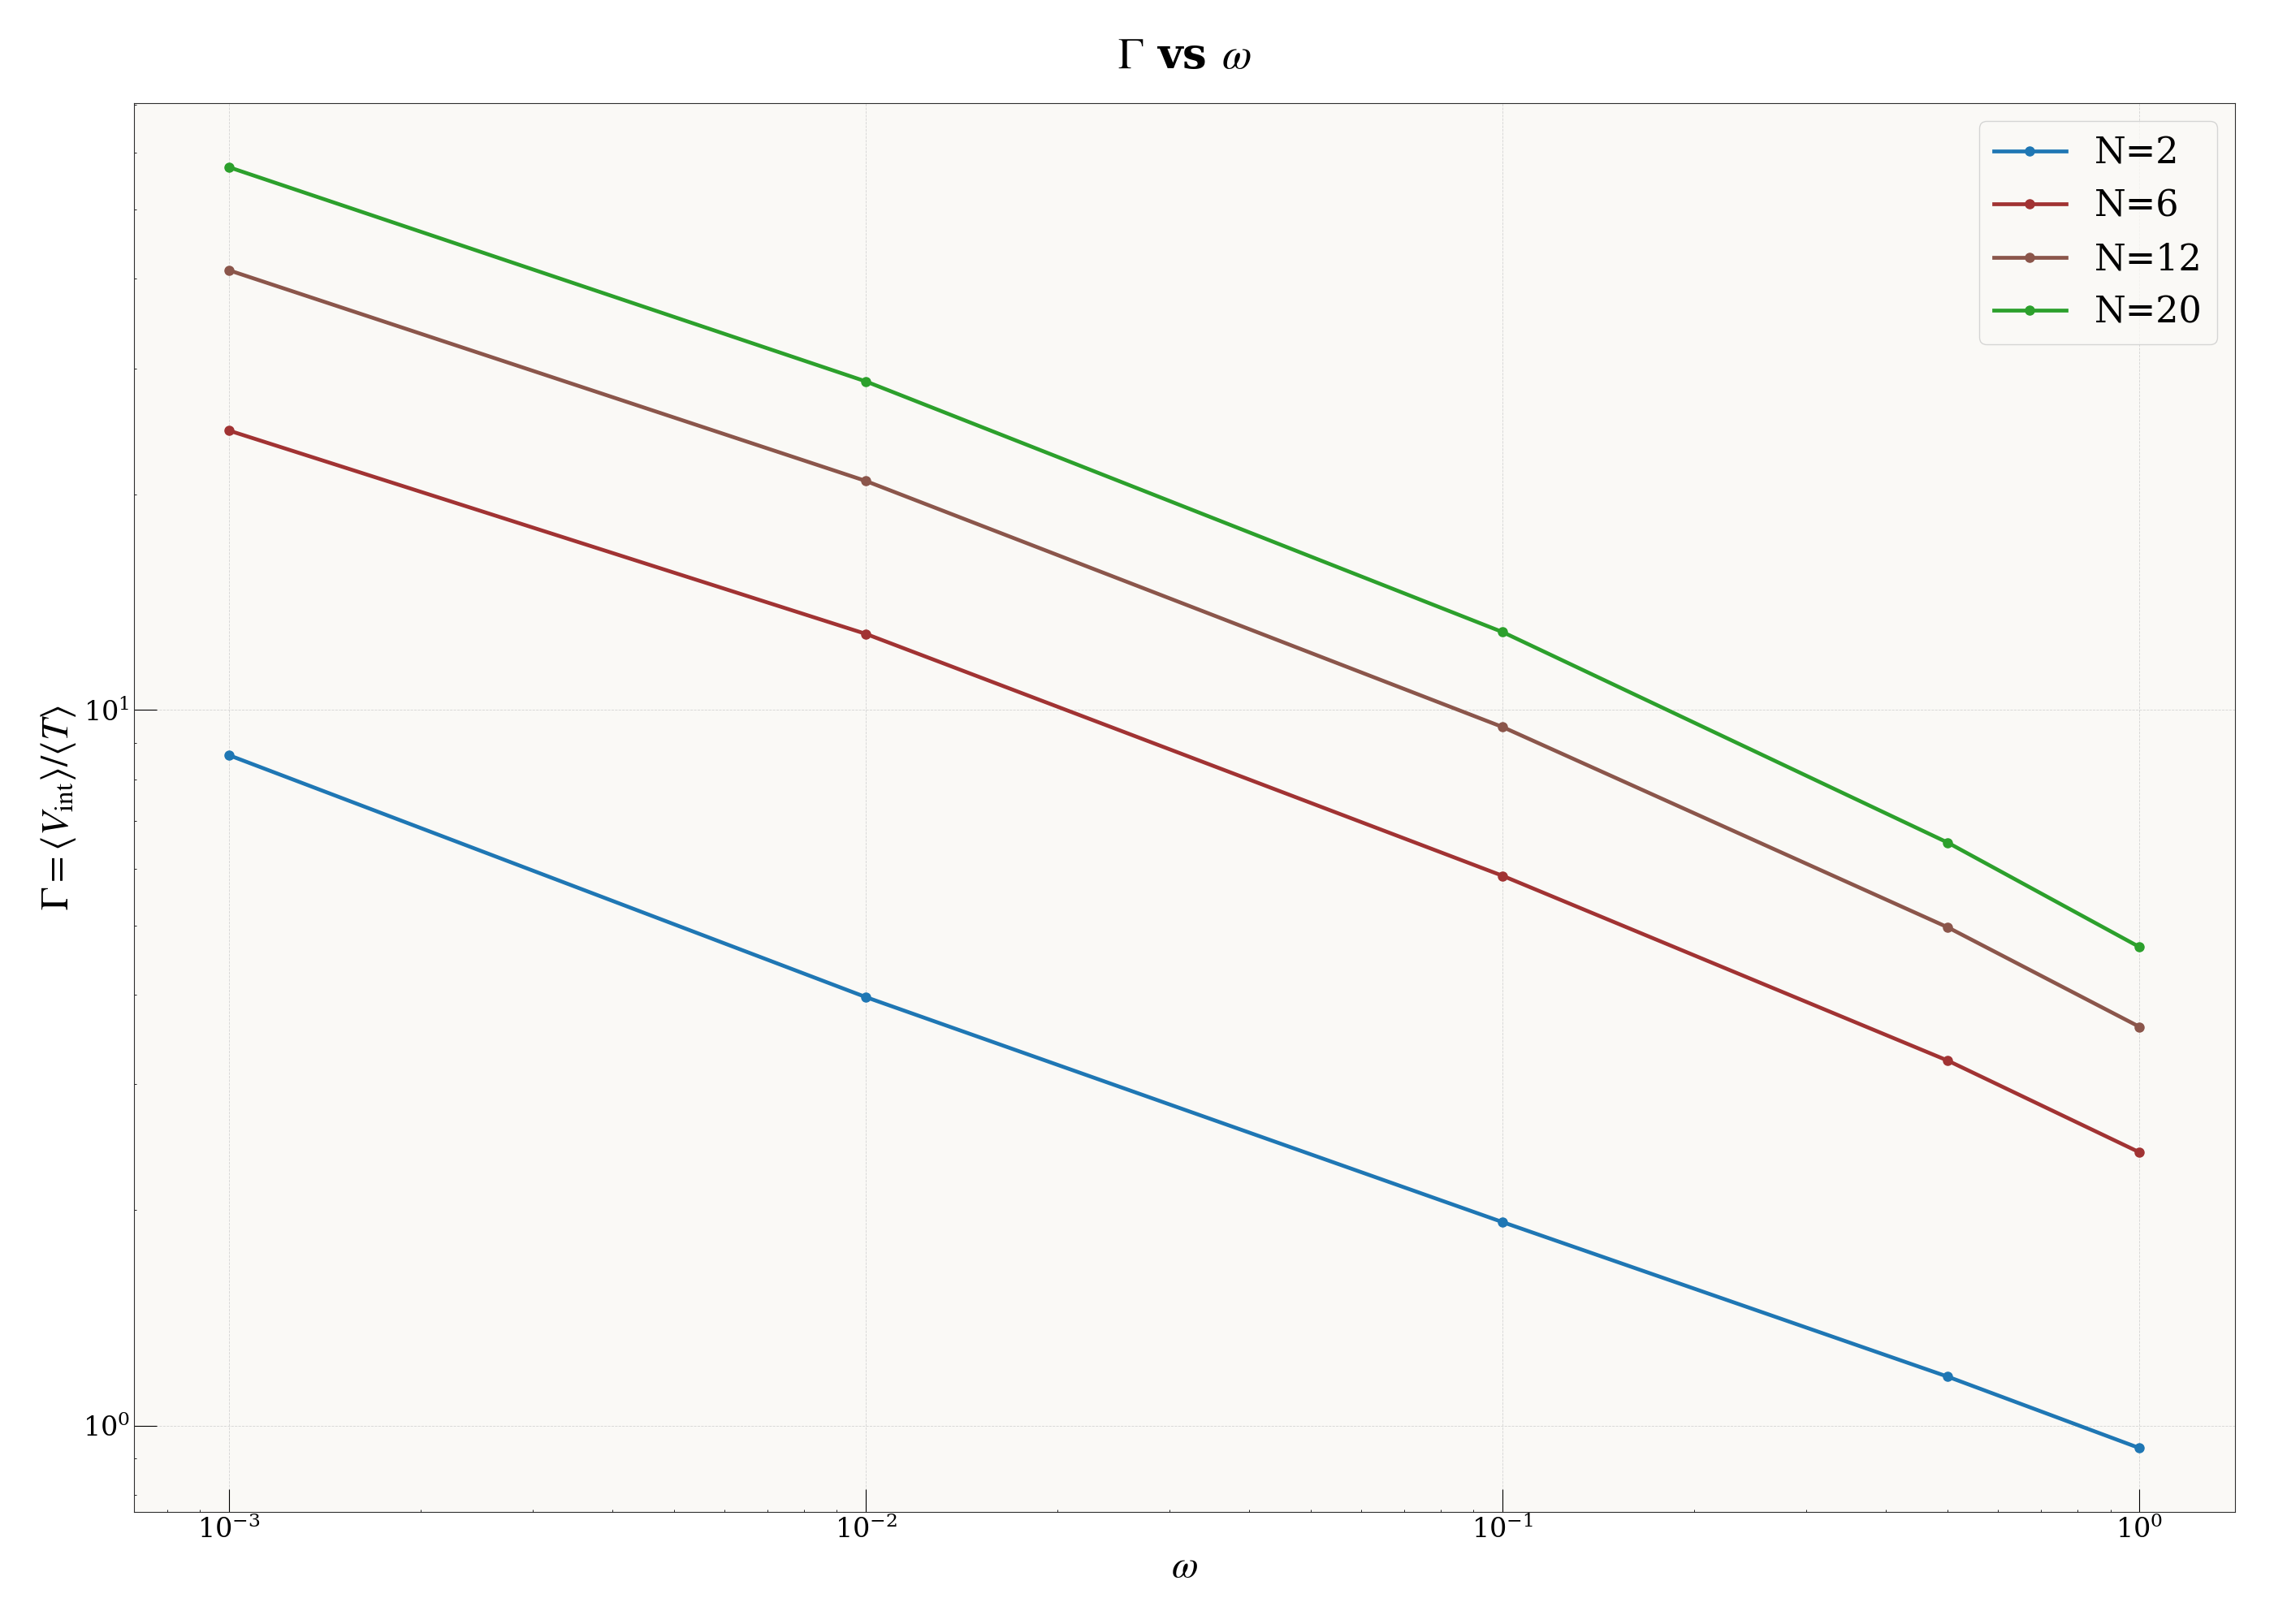
\includegraphics[width=0.48\textwidth]{figures/energy/ratios_allN_Gamma.png}}
  \hfill
  \subfloat[$\mathcal C(\omega)=2\langle V_{\rm trap}\rangle/\langle V_{\rm int}\rangle$ (horizontal line: $\mathcal C=1$).]
  {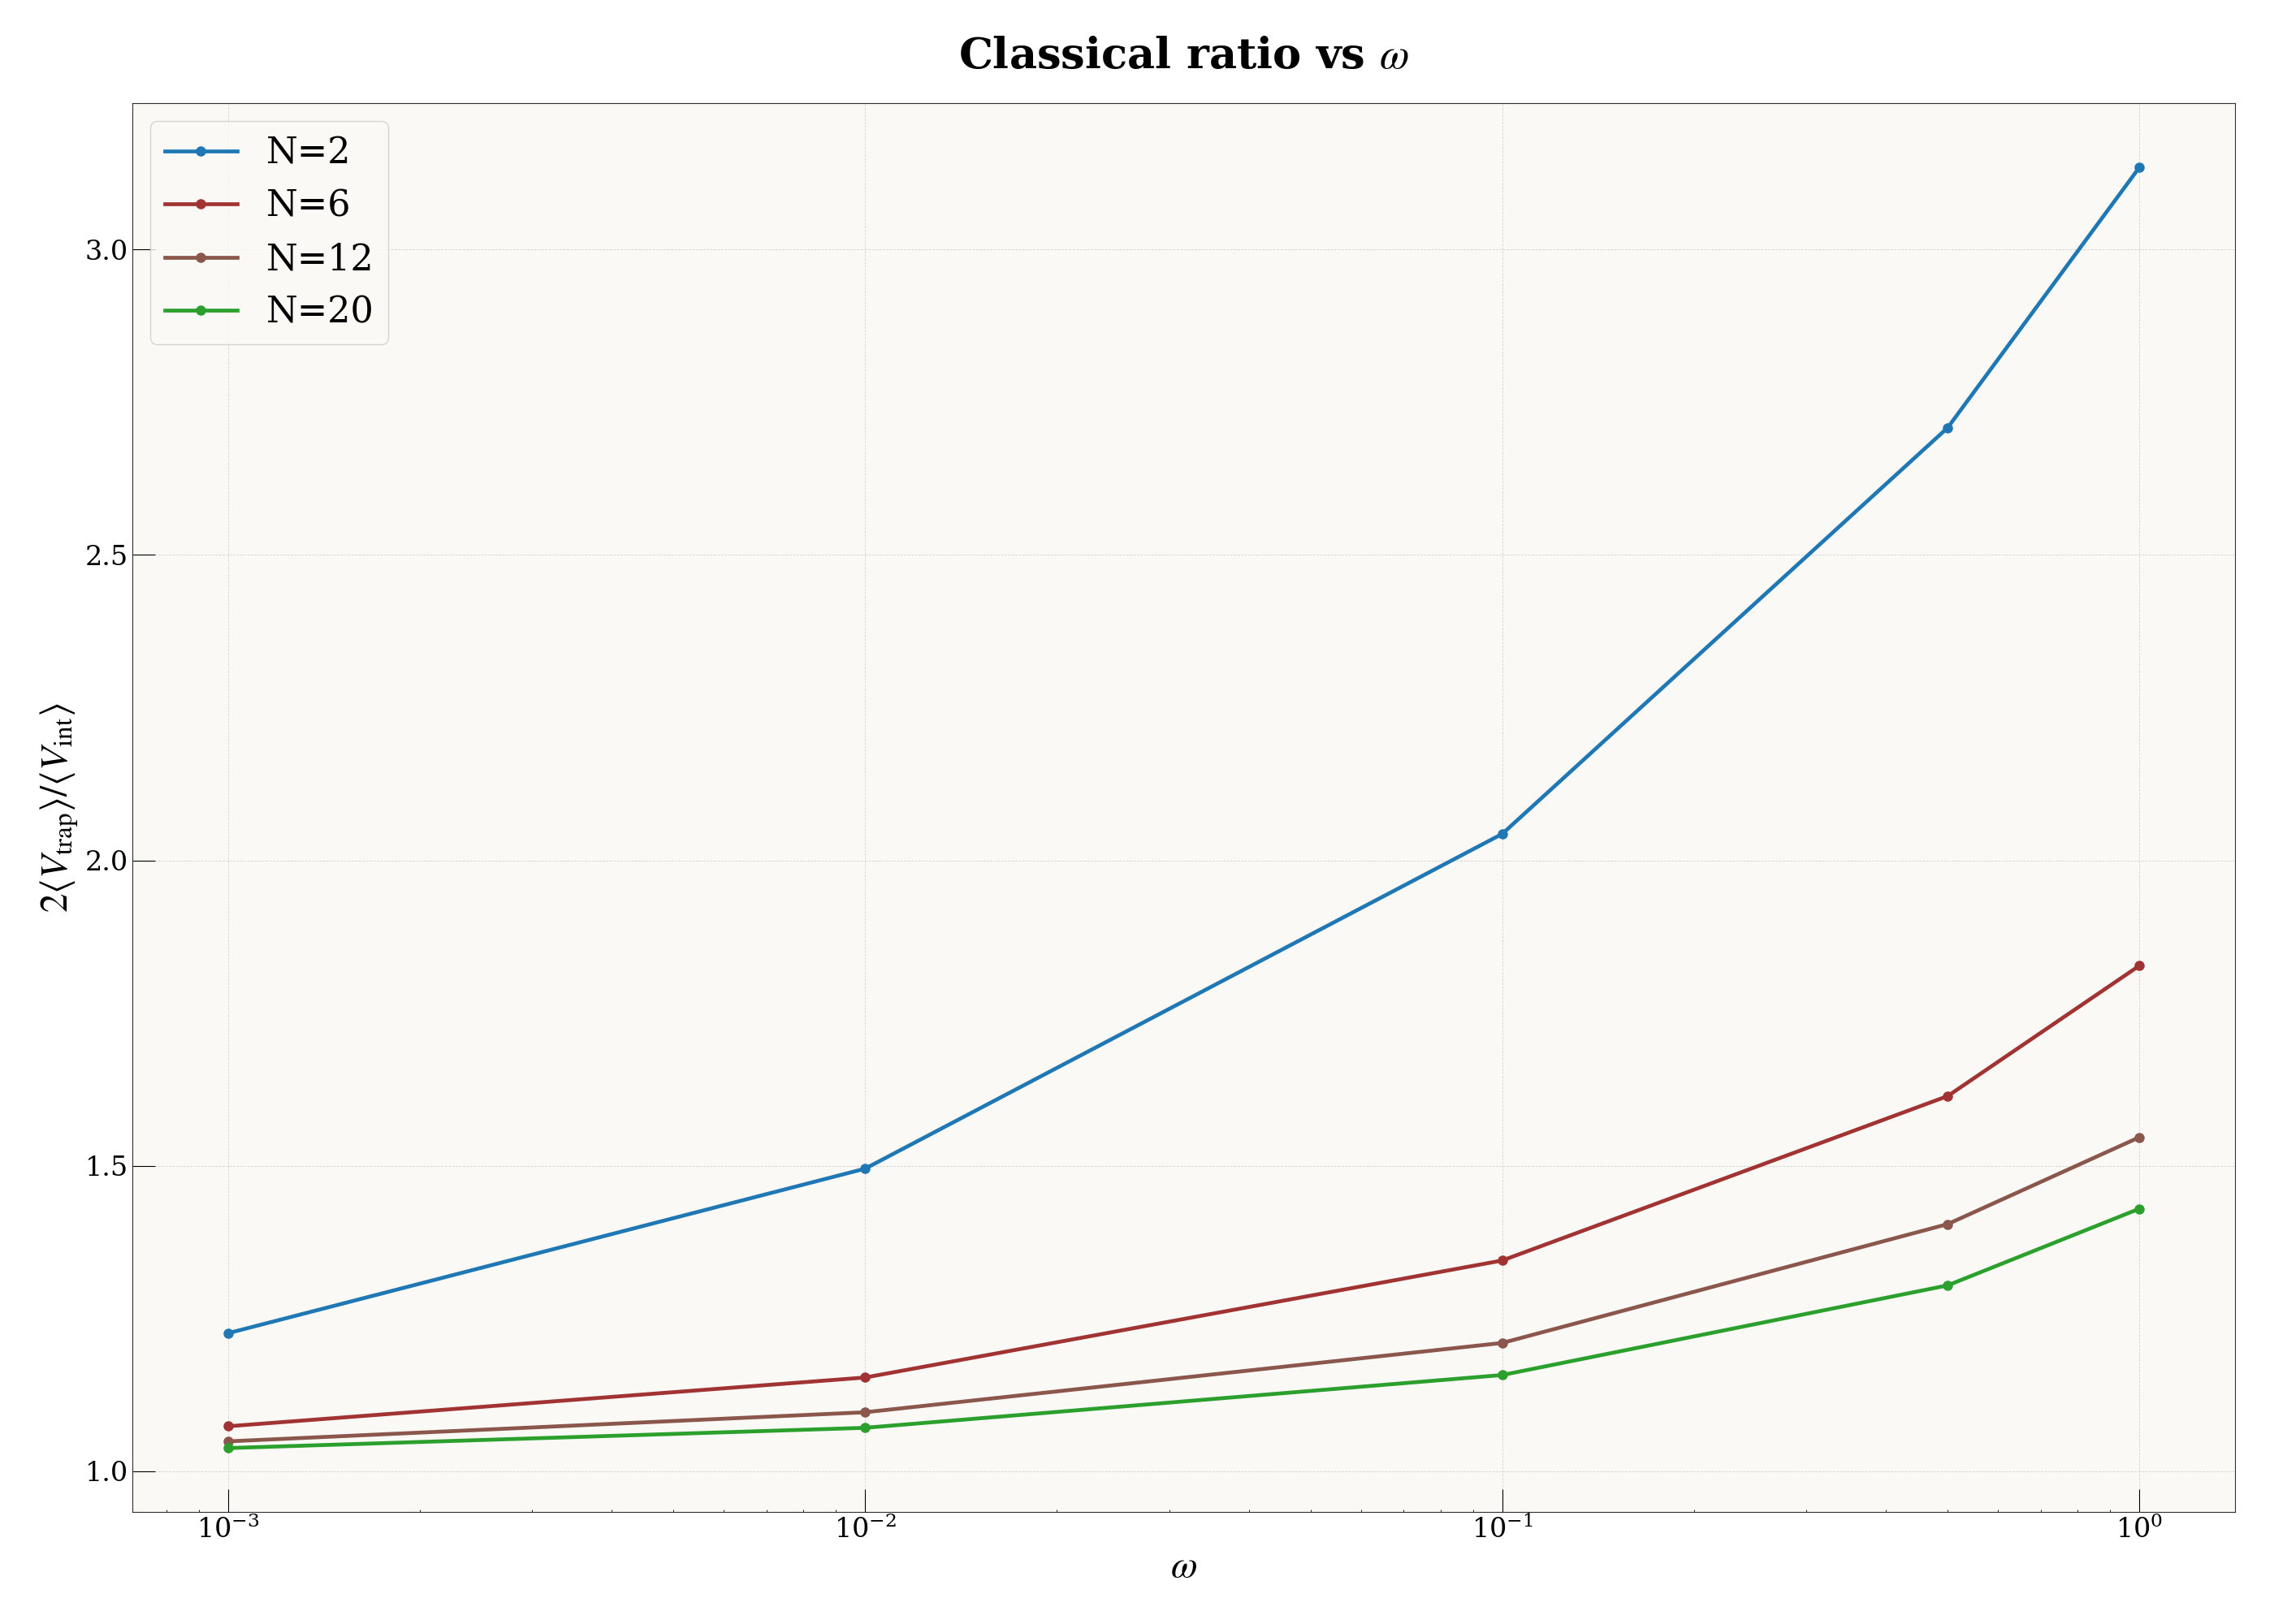
\includegraphics[width=0.48\textwidth]{figures/energy/ratios_allN_classical.png}}\\

  \caption{Energy-partition probes for the CTNN variational states.
  (a) Interaction dominance increases as confinement weakens.
  (b) The trap--Coulomb balance approaches the quasi-classical limit $\mathcal C\to 1$ at weak confinement, especially for larger $N$.
  (c) The cloud radius grows rapidly as $\omega\to 0$.
  (d) Component energies exhibit clean power-law scaling in $\omega$ on the studied grid.}
  \label{fig:energy_ratios}
\end{figure*}

% --- Table~\ref{tab:energies} (update only the N=12, omega=1 CTNN entry) ---
\begin{table*}[t]
  \centering
  \caption{Residual-based pretraining + SR tail. Reference DMC, PINN+BF and PINN+CTNN
  ground-state energies (Hartree) for selected $(N,\omega)$. Parentheses denote
  $1\sigma$ on the last digit(s). The \%\,err columns are the relative deviations
  from DMC (\%).}
  \label{tab:energies}
  \begin{threeparttable}
    \begin{tabular}{c|c|c|cc|cc}
      \toprule
      $N$ & $\omega$ & Reference (DMC) & PINN+BF & \%\,err & PINN+e & \%\,err \\
      \midrule
      2 & 0.001 & --- & $0.0137948(8)$ & --- & $\mathbf{0.013778(1)}$ & --- \\
        & 0.01 & $0.073839(2)$ & $0.073838(1)$ & $-0.0014$  & $0.0738382(5)$ & $-0.0014$ \\
        & 0.10 & $0.44079(1)$  & $0.44079(1)$  & $+0.0000$  & $0.440796(4)$ & $-0.0000$  \\
        & 0.50 & $1.65977(1)$  & $1.65976(2)$  & $-0.0006$  & $1.65976(1)$ & $-0.0006$ \\
        & 1.00 & $3.00000$     & $2.99999(1)$  & $-0.0003$  & $3.00000(2)$ & $-0.0000$  \\
      \midrule
      6 & 0.001 & ---           & $0.140913(1)$ & --- & $\mathbf{0.1408172(7)}$ & --- \\
        & 0.01 & ---            & $0.69125(2)$  & --- & $\mathbf{0.69036(1)}$ & --- \\
        & 0.10 & $3.55385(5)$   & $3.5549(1)$   & $+0.0295$ & $\mathbf{3.55388(5)}$ & $+0.0008$ \\
        & 0.50 & $11.78484(6)$  & $11.7895(4)$  & $+0.0395$  & $\mathbf{11.7847(2)}$ & $-0.0000$ \\
        & 1.00 & $20.15932(8)$  & $20.1610(6)$  & $+0.0083$  & $\mathbf{20.1585(3)}$ & $-0.0041$ \\
      \midrule
      12 & 0.001 & ---          & $0.515823(3)$ & --- & $\mathbf{0.515365(4)}$ & --- \\
         & 0.01 & ---           & $2.48620(5)$  & --- & $\mathbf{2.47363(4)}$ & --- \\
         & 0.10 & $12.26984(8)$ & $12.2731(2)$  & $+0.0160$ & $\mathbf{12.2718(1)}$ & --- \\
         & 0.50 & $39.1596(1)$  & $39.1786(8)$  & $+0.0485$ & $\mathbf{39.1604(3)}$ & $+0.0018$ \\
         & 1.00 & $65.7001(1)$  & $65.717(1)$   & $+0.0257$ & $\mathbf{65.69556(5)}$ & $-0.0069$ \\
      \midrule
      20 & 0.001 & ---          & --- & --- & $\mathbf{1.293033(6)}$ & --- \\
         & 0.01 & ---           & ---  & --- & $\mathbf{6.14645(5)}$ & --- \\
         & 0.10 & $29.9779(1)$ & ---  & --- & $29.9888(2)$ & $+0.0364$ \\
         & 0.50 & $93.8752(1)$  & ---  & --- & $\mathbf{93.8789(5)}$ & $+0.0040$ \\
         & 1.00 & $155.8822(1)$  & ---   & --- & $\mathbf{155.8738(7)}$ & $-0.0024$ \\
      \bottomrule
    \end{tabular}
  \end{threeparttable}
\end{table*}
\subsection{Wigner regime: real-space ordering and mode-based validation}
\label{subsec:Wigner}

Having established energetic accuracy in the benchmarked regimes (Table~\ref{tab:energies}), we now turn to a
structural question: \emph{what configuration do the electrons adopt in real space as confinement weakens and Coulomb
repulsion dominates?}  In a finite, rotationally symmetric trap the appropriate object is a \emph{Wigner molecule}:
electrons localize in \emph{relative} coordinates (rings/shells with polygon-like angular correlations), while the
entire pattern may rotate. Consequently, lab-frame angles can appear nearly uniform even when strong internal order
is present. We therefore combine: (i) one-body density visualization, (ii) a label-invariant shell topology, (iii)
rotation-registered bond-orientational order (internal order disentangled from lab-frame pinning), (iv) shell radii
and separation gaps, (v) a pair-statistics validation isolating angular correlations beyond shelling, and (vi) a
mode-alignment diagnostic testing whether the sampled fluctuations are consistent with structured small oscillations
around a localized configuration.

\paragraph{One-body densities (visual crossover).}
Figures~\ref{fig:onebody_w1} and~\ref{fig:onebody_w0001} compare one-body densities at strong confinement
$\omega=1.0$ and weak confinement $\omega=0.001$ for $N=2,6,12,20$. At $\omega=1.0$ the density remains compact and
the dominant change with $N$ is shell filling under the harmonic trap. At $\omega=0.001$ the density broadens
dramatically and develops pronounced radial structure for all $N$, indicating enhanced spatial separation and the
onset of Coulomb-dominated localization.



\begin{figure*}[t]
  \centering
  \subfloat[$N{=}2,\;\omega=1.0$]{%
    \densimgtwo{figures/one_body_density_2_omega_1.00000_20251029_231309.pdf}%
  }\hspace{\figgutter}%
  \subfloat[$N{=}6,\;\omega=1.0$]{%
%    \densimgtwo{figures/one_body_density_6_omega_1.00000_20251030_093439.pdf}%
  }

  \vspace{0.35em}

  \subfloat[$N{=}12,\;\omega=1.0$]{%
    \densimgtwo{figures/one_body_density_12_omega_1.00000_20251104_194000.pdf}%
  }\hspace{\figgutter}%
  \subfloat[$N{=}20,\;\omega=1.0$]{%
    \densimgtwo{figures/one_body_density_20_omega_1.00000_20251228_180301.pdf}%
  }

  \caption{One-body densities at strong confinement $\omega=1.0$ for $N=2,6,12,20$. Increasing $N$ primarily fills
  the trap while the overall extent remains compact due to the strong harmonic confinement.}
  \label{fig:onebody_w1}
\end{figure*}

\begin{figure*}[t]
  \centering
  \subfloat[$N{=}2,\;\omega=0.001$]{%
    \densimgtwo{figures/one_body_density_2_omega_0.00100_20251106_160757.pdf}%
  }\hspace{\figgutter}%
  \subfloat[$N{=}6,\;\omega=0.001$]{%
    \densimgtwo{figures/one_body_density_6_omega_0.00100_20251230_143725.pdf}%
  }

  \vspace{0.35em}

  \subfloat[$N{=}12,\;\omega=0.001$]{%
    \densimgtwo{figures/one_body_density_12_omega_0.00100_20260105_112435.pdf}%
  }\hspace{\figgutter}%
  \subfloat[$N{=}20,\;\omega=0.001$]{%
    \densimgtwo{figures/one_body_density_20_omega_0.00100_20260105_175705.pdf}%
  }

  \caption{One-body densities at weak confinement $\omega=0.001$ for $N=2,6,12,20$. The densities broaden and show
  strong radial structure, consistent with enhanced spatial separation and Wigner-molecule ordering in a
  Coulomb-dominated, low-density regime.}
  \label{fig:onebody_w0001}
\end{figure*}

\paragraph{Shell topology (discrete ring structure and where it collapses).}
To quantify radial ordering without relying on particle labels, we assign shells using a rank-based construction:
at each frame, particles are sorted by radius $r_i(t)=\|\mathbf r_i(t)\|$ and grouped into shells by fixed rank cuts.
The key qualitative information is the \emph{occupancy pattern} and where it changes. Table~\ref{tab:shell_topology_key}
summarizes only the regimes that matter structurally: the deepest Wigner case $\omega=10^{-3}$, the first post-Wigner
step $\omega=10^{-2}$ (where topology collapses for $N=12$ and $N=20$), and a representative strong-confinement point
$\omega=1$. At $\omega=10^{-3}$ we recover the expected finite-$N$ Wigner patterns: $(1,5)$ for $N=6$, $(3,9)$ for
$N=12$, and a clear three-shell structure $(1,7,12)$ for $N=20$. At $\omega=10^{-2}$, $N=12$ and $N=20$ already
collapse to $(1,11)$ and $(1,19)$, respectively, indicating a rapid loss of multi-shell localization as density
increases. For $N=6$ the two-ring pattern persists to $\omega\le 0.1$ but is no longer robust at $\omega\ge 0.5$,
where the rank-based boundary is not consistently separating and a single shell is detected.

% ============================================================
% TABLE: Shell topology (KEY regimes only)
% ============================================================
\begin{table}[t]
  \centering
  \caption{Key shell topologies (label-invariant). We report the occupancy pattern at the Wigner point
  $\omega=10^{-3}$, the first post-Wigner step $\omega=10^{-2}$, and strong confinement $\omega=1$.
  The full $\omega$ grid is consistent with these transitions.}
  \label{tab:shell_topology_key}

  \begin{threeparttable}
    \setlength{\tabcolsep}{6.2pt}
    \renewcommand{\arraystretch}{1.12}
    \begin{tabular}{c c c c}
      \toprule
      $N$ & $\omega=10^{-3}$ & $\omega=10^{-2}$ & $\omega=1$ \\
      \midrule
      2  & (2)      & (2)      & (2) \\
      6  & (1,5)    & (1,5)    & (6) \\
      12 & (3,9)    & (1,11)   & (1,11) \\
      20 & (1,7,12) & (1,19)   & (1,19) \\
      \bottomrule
    \end{tabular}
  \end{threeparttable}
\end{table}

\paragraph{Shell radii and separation gaps (quantitative localization).}
Topology tells \emph{who sits on which ring}, but the Wigner regime is also characterized by large radii and
well-separated shells. Table~\ref{tab:radii_gaps_key} reports the mean radii of the populated shells and the
inter-shell separation gaps at the same key points. In the Wigner regime ($\omega=10^{-3}$) the shell radii become
macroscopic on our scale: for $N=12$ we find $r_0\simeq 77.1$ and $r_1\simeq 189.4$ with a large separation
$\mathrm{gap}_{01}\simeq 112.3$, while $N=20$ exhibits three shells at $r_0\simeq 38.0$, $r_1\simeq 132.0$,
$r_2\simeq 247.2$ with gaps $\mathrm{gap}_{01}\simeq 94.0$ and $\mathrm{gap}_{12}\simeq 115.2$.
At $\omega=10^{-2}$ the multi-shell structures for $N=12$ and $N=20$ have already collapsed into $(1,N{-}1)$,
and the (single) separation $\mathrm{gap}_{01}$ drops accordingly, matching the topology change in
Table~\ref{tab:shell_topology_key}.

% ============================================================
% TABLE: Shell radii + gaps (KEY regimes only)
% ============================================================
\begin{table*}[t]
  \centering
  \caption{Shell radii and separation gaps at key confinement strengths (mean $\pm$ standard error over frames).
  Radii $r_s$ are reported for populated shells; $\mathrm{gap}_{01}=\langle r_1-r_0\rangle$ and
  $\mathrm{gap}_{12}=\langle r_2-r_1\rangle$. Dashes indicate non-applicable shells/gaps.}
  \label{tab:radii_gaps_key}

  \begin{threeparttable}
    \setlength{\tabcolsep}{4.2pt}
    \renewcommand{\arraystretch}{1.10}
    \begin{adjustbox}{max width=\textwidth}
    \begin{tabular}{c c c c c c c c}
      \toprule
      $N$ & $\omega$ & occ. &
      $r_0$ & $r_1$ & $r_2$ &
      $\mathrm{gap}_{01}$ & $\mathrm{gap}_{12}$ \\
      \midrule
      6  & $10^{-3}$ & (1,5)    & $35.56\pm0.21$ & $135.69\pm0.06$ & -- &
      $100.13\pm0.23$ & -- \\
      6  & $10^{-2}$ & (1,5)    & $13.348\pm0.047$ & $29.649\pm0.026$ & -- &
      $16.301\pm0.049$ & -- \\
      6  & $1$       & (6)      & $1.4996\pm0.0023$ & -- & -- &
      -- & -- \\
      \midrule
      12 & $10^{-3}$ & (3,9)    & $77.085\pm0.074$ & $189.420\pm0.047$ & -- &
      $112.335\pm0.092$ & -- \\
      12 & $10^{-2}$ & (1,11)   & $10.338\pm0.031$ & $37.662\pm0.012$ & -- &
      $27.324\pm0.028$ & -- \\
      12 & $1$       & (1,11)   & $0.5470\pm0.0022$ & $2.0020\pm0.0015$ & -- &
      $1.4550\pm0.0024$ & -- \\
      \midrule
      20 & $10^{-3}$ & (1,7,12) & $38.04\pm0.19$ & $132.033\pm0.038$ & $247.226\pm0.051$ &
      $93.99\pm0.18$ & $115.193\pm0.050$ \\
      20 & $10^{-2}$ & (1,19)   & $10.315\pm0.050$ & $44.609\pm0.012$ & -- &
      $34.294\pm0.048$ & -- \\
      20 & $1$       & (1,19)   & $0.5547\pm0.0022$ & $2.3193\pm0.0011$ & -- &
      $1.7646\pm0.0021$ & -- \\
      \bottomrule
    \end{tabular}
    \end{adjustbox}
  \end{threeparttable}
\end{table*}

\paragraph{Rotation-registered angular order (internal order vs.\ lab-frame pinning).}
Shell occupancies capture \emph{radial} localization but not whether particles on a ring exhibit polygon-like
\emph{relative} angular correlations. Because the Hamiltonian is rotationally symmetric, the correct diagnostic is
a registered (co-rotating) frame: strong internal order may coexist with a diffusing global orientation. For shell
$s$ with $n_s$ particles we compute
\begin{equation}
\psi_{n_s}^{\mathrm{reg}}(t)
=
\left|
\frac{1}{n_s}\sum_{j\in s} e^{i n_s \theta^{\mathrm{reg}}_j(t)}
\right|,
\qquad
\Phi_{s,\mathrm{reg}}=\langle \psi_{n_s}^{\mathrm{reg}} \rangle_t,
\end{equation}
and summarize internal order by
$C_{\tilde{}}\_{\mathrm{global}}=\sum_s \Phi_{s,\mathrm{reg}}$ (which can exceed unity when multiple shells are ordered).
We additionally report a lab-frame analogue $C_{\mathrm{global}}=\sum_s P_{s,\mathrm{lab}}$, which should be interpreted
as a \emph{pinning/rotation-timescale} diagnostic on the sampled time window.

Table~\ref{tab:ang_order_key} shows that internal polygonal order is strongest in the Wigner regime and collapses
rapidly when topology collapses.
For $N=12$, the Wigner case $\omega=10^{-3}$ exhibits \emph{two simultaneously ordered shells} and reaches
$C_{\tilde{}}\_{\mathrm{global}}=1.0684\pm0.0043$, while already at $\omega=10^{-2}$ (after the transition to $(1,11)$)
the internal order drops to $0.2755\pm0.0012$ and remains $\approx 0.268$ at $\omega=1$.
For $N=20$, $\omega=10^{-3}$ again shows multi-shell internal order with $C_{\tilde{}}\_{\mathrm{global}}=0.7909\pm0.0027$,
whereas the collapsed $(1,19)$ states have $C_{\tilde{}}\_{\mathrm{global}}\simeq 0.203$ at $\omega\ge 10^{-2}$.
In all cases, $C_{\mathrm{global}}$ is much smaller than $C_{\tilde{}}\_{\mathrm{global}}$, consistent with weak
lab-frame pinning and substantial global rotation over the sampled trajectories.

% ============================================================
% TABLE: Angular order (KEY regimes only)
% ============================================================
\begin{table}[t]
  \centering
  \caption{Rotation-registered (internal) vs.\ lab-frame (pinning) angular order at key confinement strengths.
  $C_{\tilde{}}\_{\mathrm{global}}$ measures internal polygonal order in the registered frame, while $C_{\mathrm{global}}$
  quantifies residual lab-frame pinning on the sampled time window. Uncertainties are standard errors over frames.}
  \label{tab:ang_order_key}

  \begin{threeparttable}
    \setlength{\tabcolsep}{5.8pt}
    \renewcommand{\arraystretch}{1.12}
    \begin{tabular}{c c c c c}
      \toprule
      $N$ & $\omega$ & occ. & $C_{\tilde{}}\_{\mathrm{global}}$ & $C_{\mathrm{global}}$ \\
      \midrule
      2  & $10^{-3}$ & (2)      & $0.8746\pm0.0012$ & $0.0066\pm0.0041$ \\
      2  & $10^{-2}$ & (2)      & $0.7576\pm0.0024$ & $0.0066\pm0.0034$ \\
      2  & $1$       & (2)      & $0.6283\pm0.0028$ & $0.0034\pm0.0020$ \\
      \midrule
      6  & $10^{-3}$ & (1,5)    & $0.6520\pm0.0020$ & $0.0095\pm0.0033$ \\
      6  & $10^{-2}$ & (1,5)    & $0.4340\pm0.0017$ & $0.0041\pm0.0022$ \\
      6  & $1$       & (6)      & $0.3656\pm0.0013$ & $0.0042\pm0.0018$ \\
      \midrule
      12 & $10^{-3}$ & (3,9)    & $1.0684\pm0.0043$ & $0.0206\pm0.0048$ \\
      12 & $10^{-2}$ & (1,11)   & $0.2755\pm0.0012$ & $0.0046\pm0.0015$ \\
      12 & $1$       & (1,11)   & $0.2678\pm0.0014$ & $0.0032\pm0.0013$ \\
      \midrule
      20 & $10^{-3}$ & (1,7,12) & $0.7909\pm0.0027$ & $0.0560\pm0.0040$ \\
      20 & $10^{-2}$ & (1,19)   & $0.2032\pm0.0008$ & $0.0004\pm0.0007$ \\
      20 & $1$       & (1,19)   & $0.2027\pm0.0010$ & $0.0030\pm0.0010$ \\
      \bottomrule
    \end{tabular}
  \end{threeparttable}
\end{table}

\paragraph{Lindemann-type disorder (progressive melting with confinement).}
To complement angular order parameters we track a registered Lindemann-type measure $L_{s,\mathrm{reg}}$ per shell,
which quantifies the size of relative positional fluctuations compared to the shell scale (larger means more disordered).
Table~\ref{tab:lindemann_key} shows a consistent monotonic melting trend: weak confinement produces stiff rings, while
strong confinement produces substantially larger relative fluctuations. For $N=12$ and $N=20$ the Wigner point
$\omega=10^{-3}$ exhibits \emph{simultaneously stiff multiple shells} (e.g.\ $N=12$: $L_{\mathrm{in,reg}}=0.2736\pm0.0013$,
$L_{\mathrm{out,reg}}=0.2547\pm0.0010$; $N=20$: $L_{7,\mathrm{reg}}=0.3514\pm0.0008$, $L_{12,\mathrm{reg}}=0.2696\pm0.0007$),
while after collapse to $(1,N{-}1)$ the outer shell becomes increasingly disordered, reaching $0.6178\pm0.0010$ for
$N=12$ and $0.6920\pm0.0010$ for $N=20$ at $\omega=1$.

% ============================================================
% TABLE: Lindemann disorder (KEY regimes only)
% ============================================================
\begin{table}[t]
  \centering
  \caption{Registered Lindemann-type disorder at key confinement strengths (mean $\pm$ standard error over frames).
  For multi-shell Wigner states, both inner and outer shells are shown. Dashes indicate non-applicable shells.}
  \label{tab:lindemann_key}

  \begin{threeparttable}
    \setlength{\tabcolsep}{6.2pt}
    \renewcommand{\arraystretch}{1.12}
    \begin{tabular}{c c c c c}
      \toprule
      $N$ & $\omega$ & occ. & $L_{\mathrm{in,reg}}$ & $L_{\mathrm{out,reg}}$ \\
      \midrule
      2  & $10^{-3}$ & (2)      & --                & $0.1325\pm0.0007$ \\
      2  & $10^{-2}$ & (2)      & --                & $0.2046\pm0.0014$ \\
      2  & $1$       & (2)      & --                & $0.4004\pm0.0022$ \\
      \midrule
      6  & $10^{-3}$ & (1,5)    & --                & $0.2049\pm0.0008$ \\
      6  & $10^{-2}$ & (1,5)    & --                & $0.3443\pm0.0011$ \\
      6  & $1$       & (6)      & --                & $0.5607\pm0.0011$ \\
      \midrule
      12 & $10^{-3}$ & (3,9)    & $0.2736\pm0.0013$ & $0.2547\pm0.0010$ \\
      12 & $10^{-2}$ & (1,11)   & --                & $0.4500\pm0.0010$ \\
      12 & $1$       & (1,11)   & --                & $0.6178\pm0.0010$ \\
      \midrule
      20 & $10^{-3}$ & (1,7,12) & $0.3514\pm0.0008$ & $0.2696\pm0.0007$ \\
      20 & $10^{-2}$ & (1,19)   & --                & $0.5716\pm0.0011$ \\
      20 & $1$       & (1,19)   & --                & $0.6920\pm0.0010$ \\
      \bottomrule
    \end{tabular}
  \end{threeparttable}
\end{table}

\paragraph{Mode-alignment diagnostic (are the fluctuations ``molecule-like''?).}
A Wigner molecule is not merely a static ring pattern: if electrons are localized around a classical equilibrium,
their residual motion should resemble structured small oscillations (collective distortions) rather than featureless
fluid-like wandering. We test this by comparing the empirical covariance $C$ (center-of-mass removed) to the Hessian
$H$ of the corresponding classical equilibrium configuration (trap + Coulomb, scaled to the same $\omega$). If
fluctuations are organized by classical normal modes, $C$ and $H$ should be approximately compatible (near joint
diagonalization) and a nontrivial fraction of variance should lie in the span of the softest modes. The diagnostics
in Table~\ref{tab:classical_mode_alignment} support this interpretation: for $N=6$ the commutator norm is smallest at
$\omega=10^{-3}$ and increases with confinement, while for $N=12$ and $N=20$ the commutator norms remain small and
overlap weights show a reproducible concentration of variance into a soft-mode subspace even though the fluctuation
space is high-dimensional.

% ============================================================
% TABLE: Classical-mode alignment + concentration
% (insert your existing Table~\ref{tab:classical_mode_alignment} here unchanged)
% ============================================================

\paragraph{Pair-statistics validation (angular order beyond shelling).}
Shell topology captures the dominant radial organization, but it does not by itself guarantee polygon-like angular
correlations. We therefore compare the empirical global pair-distance histogram to two shell-based generative models
sharing the \emph{same} shell assignment: (i) a polygon model (regular $n_s$-gons per shell with optimal phase alignment)
and (ii) a uniform-angle model (same shell radii but no angular order). Table~\ref{tab:shell_pair_model_validation}
shows that the polygon model systematically outperforms the uniform-angle baseline, and that the gain
$\Delta\cos=\cos_{\mathrm{poly}}-\cos_{\mathrm{uni}}$ is strongest in the weakest trap and decreases with $\omega$,
isolating a genuine angular-correlation signal beyond radial shelling alone.

% ============================================================
% TABLE: Pair-distance model validation (polygon vs uniform)
% (insert your existing Table~\ref{tab:shell_pair_model_validation} here unchanged)
% ============================================================

\paragraph{Discussion (what the combined diagnostics establish).}
Across $N=2,6,12,20$ we observe a consistent and internally validated Wigner-to-denser structural crossover as $\omega$
decreases. The one-body densities show dramatic spatial expansion and ring formation at $\omega=10^{-3}$.
The shell topology reveals \emph{discrete} finite-$N$ Wigner patterns at $\omega=10^{-3}$ and sharp collapses at
$\omega=10^{-2}$ for $N=12$ and $N=20$. The shell radii and separation gaps provide a quantitative real-space
counterpart: in the Wigner regime the shells are widely separated and stable, while their radii and gaps shrink
rapidly as confinement strengthens. Rotation-registered bond-orientational order demonstrates strong polygon-like
internal angular localization in the Wigner regime (including multi-shell ordering for $N=12$ and $N=20$), while the
lab-frame measures remain comparatively small and should be interpreted as pinning/rotation-timescale diagnostics
rather than internal order. The Lindemann measures rise strongly with confinement, giving an independent signature of
progressive melting. Finally, the pair-distance validation confirms that angular correlations contribute explanatory
power beyond shelling, with the largest gains at weak confinement, and the mode-alignment analysis adds mechanistic
support: in the low-$\omega$ regime the fluctuations retain structured, collective content compatible with
small-oscillation physics around localized configurations, as expected for Wigner molecules in a finite trap.
\section{Conclusion and Perspectives}



\bibliography{apssamp}% Produces the bibliography via BibTeX.
\end{document}
